% !TEX encoding = UTF-8 Unicode
\documentclass[dvipsnames]{beamer}
\usepackage[brazil]{babel}
\usepackage[T1]{fontenc}
%\usepackage[latin1]{inputenc}
\usepackage[utf8x]{inputenc}
\usepackage[ruled,linesnumbered,vlined,boxed]{algorithm2e}

\usepackage{color,colortbl}


\usepackage{multirow}

\mode<presentation>
{
        \usetheme{Frankfurt}

        \setbeamercovered{transparent}
        \setbeamertemplate{theorems}[numbered]
}

%\usepackage[english]{babel}
%\usepackage[brazil]{babel}
%
%%\usepackage[utf8]{inputenc}
%\usepackage[latin1]{inputenc}
%\usepackage[T1]{fontenc}

\usepackage{times}

\usepackage{moreverb}
\usepackage{verbatim}

\usepackage{hyperref}

\usepackage{amsmath}

\newcommand{\dist}{{\rm dist}}

\usepackage[mathscr]{euscript}

\usepackage{graphicx}
\usepackage{color}

\newtheorem{observation}{Observation}
\newtheorem{proposition}{Proposition}

\newcommand{\inputG}{\widehat{G}}
\newcommand{\finalT}{\widehat{T}}
\newcommand{\inputM}{\widehat{\delta}}
\newcommand{\finalM}{\widehat{\tau}}
\newcommand{\intersec}{\mathcal{I}}
\newcommand{\forest}{\mathcal{F}}
\newcommand{\partition}{\mathcal{P}}
\newcommand{\external}{\overline{E}}
\newcommand{\transitive}{\mathcal{R}}
%\newcommand{\N}{\mathbb{N}}
%\newcommand{\R}{\mathbb{R}}

\usepackage{color}
\usepackage{xcolor}

\usepackage{lipsum}
%\newcommand\Fontvi{\fontsize{8}{7.2}\selectfont}
\newcommand\Fontvimaior{\fontsize{8}{7.2}\selectfont}

\newtheorem{fato}{Fato}
\newtheorem*{defi}{Definição}
\newtheorem*{propri}{Propriedades}
\newtheorem*{prop}{Proposição}
 \newtheorem{ex}{Exercício}
%\newtheorem{theorem}{Teorema}[section]
\newtheorem{conjecture}{Conjectura}
\newtheorem{definicao}{Definição}
\newtheorem{notacao}{Notação}
\newtheorem{teorema}{Teorema}
%\newtheorem{proposition}{Proposition}
\newtheorem{afirmacao}{Afirmação}[teorema]
\newtheorem{lema}{Lema}
\newtheorem{observacao}{Observação}
%\newtheorem{proposicao}{Proposição}[section]
\newtheorem{proposicao}{Proposição}
%\newtheorem{corolario}{CorolÁrio}[section]
\newtheorem{corolario}{Corolário}
\newtheorem{conjectura}{Conjectura}
\newtheorem{problema}{Problema}
\newtheorem{exemplo}{Exemplo}
%----------------------------


\newcommand{\espacoXBinary}{\{0,1\}^{|E|}}
\newcommand{\espacoUuni}{\mathbb{R}^{|V|}}
\newcommand{\espacoZBinary}{\{0,1\}^{2|E|}}
\newcommand\Fontvi{\fontsize{5}{6.2}\selectfont}


\newcommand{\espacoU}{\mathbb{R}^{|V| \times |V|}}
\newcommand{\espacoUr}{\mathbb{R}^{|V|}}
\newcommand{\Tscr}{\mathscr{T}}
\newcommand{\Pscr}{\mathscr{P}}
\newcommand{\Pcal}{\mathcal{P}}
%\newcommand{\dist}{{\rm dist}}
\newcommand{\R}{\mathbb{R}}
\newcommand{\Z}{\mathbb{Z}}
\newcommand{\B}{\mathbb{B}}
\newcommand{\N}{\mathbb{N}}
\newcommand{\Q}{\mathbb{Q}}
\newcommand{\Ccal}{\mathscr{C}}
\newcommand{\NP}{\mathscr{NP}}
\newcommand{\DTIME}{\mathscr{DTIME}}
\newcommand{\classeP}{\mathscr{P}}	
\newcommand{\littleO}{o}
\newcommand{\bigO}{\mathcal{O}}
\newcommand{\RC}{\textsc{RC}}
\newcommand{\CR}{\textsc{CR}}
\newcommand{\ExtColr}{\text{r-\textsc{ExtCol}}}
\newcommand{\ExtCol}{\textsc{1-ExtCol}}
\newcommand{\RCp}{\textsc{RC-param}}
\newcommand{\RCA}{\textsc{RCA}}
\newcommand{\RCum}{\textsc{RC-bin}}
\newcommand{\REC}{\mathscr{R}}
\newcommand{\RECA}{\mathscr{T}} 
\newcommand{\affinerank}{\rm affinerank}
\newcommand{\rank}{{\rm rank}}
\newcommand{\affine}{{\rm affine}}
\newcommand{\conv}{{\rm conv} }
\newcommand{\V}{\chi}
\newcommand{\poli}{\mathcal{P}}
\newcommand{\npd}{\mathcal{NPD}}
\newcommand{\npc}{\mathcal{NPC}}
\newcommand{\fpt}{\mathcal{FPT}}
\newcommand{\poliQ}{\mathcal{Q}}
\newcommand{\CRT}{\textsc{CRT}}
%----------------------------
%\usepackage[pdftex]{graphicx} %pacote que esta dando problema
\usepackage{pdfpages}
\usepackage{newclude}
\usepackage[mathscr]{euscript}
%----------------------------
 %% \setlength{\textwidth}{35pc}
 %% \setlength{\oddsidemargin}{1.25cm}
 %% \setlength{\evensidemargin}{1.25cm} 
\graphicspath{{./figuras/}}
%----------------------------
\DeclareMathOperator*{\argmin}{arg\,min}
%----------------------------
%comandos para novas letras/exppressões
\newcommand{\incid}{\mathcal{X}}
\newcommand{\incidY}{\mathcal{Y}}
\newcommand{\maxstretchfactor}{\mathcal{T}}
\newcommand{\espacoX}{\mathbb{R}^{|E|}}
\newcommand{\espacoY}{\mathbb{R}^{|E| \times |E|}}
\newcommand{\PGtrestricoes}{\rm{(PL)}}
\newcommand{\facetF}{\mathcal{F}}
\newcommand{\maxcam}{{\rm maxCam}}
%----------------------------
%LP formulation
\usepackage{lpform} %LPs
\renewcommand{\lpforall}[1]{&& \forall #1}
%----------------------------
%rescaling letters
\usepackage{mathrsfs} %mathscr
% \newcommand{\smallG}{\mbox{\larger[-1]$(G)$}}
% \newcommand{\smallGf}{\mbox{\larger[-1]$(G-f)$}}
% \newcommand{\smallGprime}{\mbox{\larger[-1]$(G')$}}
% \newcommand{\smallGprimef}{\mbox{\larger[-1]$(G'-f)$}}
% \newcommand{\smallGprimeG}{\mbox{\larger[-1]$(G',G)$}}
% \newcommand{\smallW}{\mbox{\larger[-1]$(G[W])$}}
% \newcommand{\smallWg}{\mbox{\larger[-1]$(G[W]-g)$}}
% \newcommand{\smallWWbarf}{\mbox{\larger[-1]$(G[E(W) \cup E(\overline{W})+f])$}}
% \newcommand{\smallWWbarfg}{\mbox{\larger[-1]$(G[E(W) \cup E(\overline{W})+f-g])$}}
% \newcommand{\smallH}{\mbox{\larger[-1]$(H)$}}
% \newcommand{\smallF}{\mbox{\larger[-1]$(G[F])$}}

\newcommand{\smallG}{\mbox{$(G)$}}
\newcommand{\smallGf}{\mbox{$(G-f)$}}
\newcommand{\smallGprime}{\mbox{$(G')$}}
\newcommand{\smallGprimef}{\mbox{$(G'-f)$}}
\newcommand{\smallGprimeG}{\mbox{$(G',G)$}}
\newcommand{\smallW}{\mbox{$(G[W])$}}
\newcommand{\smallWg}{\mbox{$(G[W]-g)$}}
\newcommand{\smallWWbarf}{\mbox{$(G[E(W) \cup E(\overline{W})+f])$}}
\newcommand{\smallWWbarfg}{\mbox{$(G[E(W) \cup E(\overline{W})+f-g])$}}
\newcommand{\smallH}{\mbox{$(H)$}}
\newcommand{\smallF}{\mbox{$(G[F])$}}

\newcommand{\spanPath}{\mathcal{P}}
\newcommand{\spanBridge}{\mathcal{B}}
\newcommand{\Pathuv}{\spanPath_{u,v}^{t}}
\newcommand{\Pathpq}{\spanPath_{p,q}^{t}}
\newcommand{\Path}{\spanPath^{t}}
\newcommand{\PathuvF}{\Pathuv\smallF}
\newcommand{\PathuvG}{\Pathuv\smallG}
\newcommand{\PathuvH}{\Pathuv\smallH}
\newcommand{\PathuvGprime}{\Pathuv\smallGprime}
\newcommand{\PathuvGf}{\Pathuv\smallGf}
\newcommand{\PathuvGprimef}{\Pathuv\smallGprimef}
\newcommand{\PathpqW}{\Pathpq\smallW}
\newcommand{\PathpqWg}{\Pathpq\smallWg}
\newcommand{\PathpqWWbarf}{\Pathpq\smallWWbarf}
\newcommand{\PathpqWWbarfg}{\Pathpq\smallWWbarfg}
\newcommand{\BridgeuvPrime}{\spanBridge_{u',v'}^{t}}
\newcommand{\BridgeuvPrimeG}{\spanBridge_{u',v'}^{t}(G)}
\newcommand{\Bridgeuv}{\spanBridge_{u,v}^{t}}
\newcommand{\BridgeuvG}{\spanBridge_{u,v}^{t}(G)}
\newcommand{\Bridge}{\spanBridge^{t}}
\newcommand{\BridgeG}{\spanBridge^{t}(G)}
%\newcommand{\smallQBridge}{\mbox{\larger[-1]$(Q \cup \Bridge)$}}%%%%% yw mudou
\newcommand{\smallQBridge}{\mbox{$(Q \cup \Bridge)$}}%%%%% yw new
\newcommand{\PathuvQBridge}{\Pathuv\smallQBridge}
\newcommand{\BridgeuvGprime}{\Bridgeuv\smallGprime}
\newcommand{\BridgeuvPrimeGf}{\spanBridge_{u',v'}^{t}\smallGf}
\newcommand{\BridgeuvGf}{\Bridgeuv\smallGf}
\newcommand{\BridgeGf}{\Bridge\smallGf}
\newcommand{\BridgeuvGprimeG}{\Bridgeuv\smallGprimeG}
\newcommand{\BridgeTwo}{\spanBridge_{2}^{t}}
\newcommand{\BridgeGprime}{\Bridge\smallGprime}
\newcommand{\BridgeTwoGprime}{\BridgeTwo\smallGprime}
\newcommand{\BridgeTwoGf}{\BridgeTwo\smallGf}
%----------------------------


\title[Spanners]
{Árvore Spanner de Custo Mínimo}

\author[hugo]
{Hugo Braga}

\institute[USP]
{
 %Doutorando em Ci\^{e}ncia da Computa\c{c}\~{a}o\\
 Instituto de Matem\'{a}tica e Estat\'{i}stica\\
 Universidade de S\~{a}o Paulo\\
 %Orientadora: Prof. Yoshiko Wakabayashi
}

\date[Short Occasion]
{II Encontro de Teoria da Computação \\ 04 de Julho de 2017  }

\subject{Talks}

\begin{document}

\begin{frame}
 \titlepage
\end{frame}

%% \begin{frame}{Agenda}
%%   \tableofcontents
%%   % You might wish to add the option [pausesections]
%% \end{frame}

\section{Introdução}

\begin{frame}{Definição}

\begin{itemize}
 \item $G$ grafo conexo. $u,v \in V(G)$.\\
   $H \subseteq G$ subgrafo gerador de $G$.\\
   Custos $w: E(G) \rightarrow \R^+$.\\
   real $t > 1$.
 \item $H$ \textcolor{red}{\emph{spanner}} de $G$ se 

\begin{equation}
  \dist_{H}(u,v) \le t \cdot \dist_{G}(u,v), \quad \forall\;u,v \in V,
  \label{eq:def_spanner}
\end{equation}

%% \end{itemize}
%% \end{frame}

%% \begin{equation*}
%% str_{H,G}(u,v) = \frac{dist_{H}(u,v)}{dist_{G}(u,v)}.
%% \end{equation*}
%% \label{eq:def_spanner}

\item Exemplo (com custo unitário):

\begin{minipage}[t][.5\textheight][t]{\textwidth}
%\begin{figure}[H]
\centering
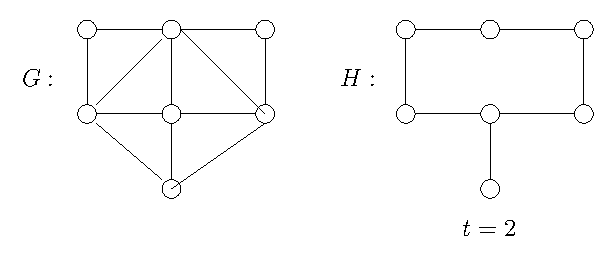
\includegraphics[scale=0.55]{figures/stretch_example_w_label.eps}
%\label{fig:fig1}
%\end{figure}
\end{minipage}

\end{itemize}

\end{frame}

\begin{frame}{Árvore $t$-spanner}
\begin{itemize}

 \item $H$ é uma árvore $\rightarrow H$ é uma \textcolor{red}{\emph{árvore t-spanner}} de $G$.

\begin{figure}[H]
\centering
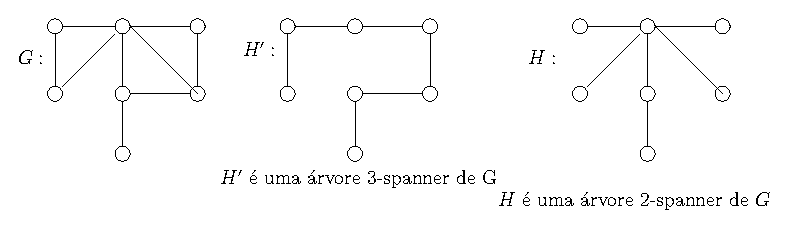
\includegraphics[scale=0.65]{figures/arvore_spanner.eps}
\label{fig:fig1}
\end{figure}

\end{itemize}
\end{frame}


\section{Background}
\begin{frame}{Problema central}
  \begin{itemize}
    \item Árvore $t$-spanner de custo mínimo (MWTS):\\
      Dado $G=(V,E)$, (real) $t > 1$ e $w: E \rightarrow \R^{+}$, \\
      % Dado um grafo $G=(V,E)$, um (real) $t$ e $w(E) \rightarrow \R^{+}$, é possível 
    encontrar uma árvore $t$-spanner em $G$ de custo mínimo.
    %\item <2->Custo unitário $\rightarrow$ problema de \emph{spanner esparsa}.
  \end{itemize}
\end{frame}

%% \begin{frame}{Problemas sobre spanners}
%%   \begin{itemize}
%%     \item Árvore spanner de dilatação mínima:\\
%%       $G=(V,E)$ e $w(E) \rightarrow \R^{+}$\\
%%       Qual o menor $t$ t.q. $G$ contém um $t$-spanner?
%%   \end{itemize}
%% \end{frame}

%% \begin{frame}{Problemas sobre spanners}
%%   \begin{itemize}
%%     \item <1->$t$-spanner de custo mínimo:\\
%%       $G=(V,E)$, (real) $t$ e $w(E) \rightarrow \R^{+}$.\\
%%       Encontrar um $t$-spanner de $G$ de custo mínimo.
%%     \item <2->Custo unitário $\rightarrow$ problema de \emph{spanner esparsa}.
%%   \end{itemize}
%% \end{frame}

\begin{frame}{Histórico}
  \begin{itemize}
%    \item <1-> Chew, 1986: Presented the problem of approximating complete euclidean graphs by planar subgraphs.% \cite{Chew1986}.
    \item Peleg \& Ullman, 1987: noção de spanner.
%was introduced by Peleg and Ullman \cite{PelegU1987} 
%to build synchronizers.
    \item Peleg \& Sch\"{a}ffer, 1989: spanner esparsa.
% were first studied in \cite{PelegS1989}. 
%         \begin{itemize}
%           \item For $t = 2$, the sparse spanner is NP-complete.
%           \item Polynomial algorithm to build a $(4t + 1)$-spanner with $O(n^{1+1/t})$ 
% edges, for $t \ge 1$ (arbitrary graphs).
%         \end{itemize}
%    \item Alth\"{o}fer et al., 1993: esparsidade $x$ fator de dilatação.
% for constructing $(2t + 1)$-spanner with at most 
% $n\lceil n^{1/t}  \rceil$ edges.
% %, for $t \ge 1$ (arbitrary weighted graphs).% \cite{AlthoferDDJS1993}.
%       \begin{itemize}
%         \item The spanner has low weight.
%       \end{itemize}
  \end{itemize}
\end{frame}

%% \begin{frame}{Aplicação}
%%   \begin{itemize}
%%    \item <1->Sistemas distribuídos.
%%    \item <2->Redes de comunicação.
%%   \end{itemize}
%% \end{frame}


% \begin{frame}{Research on Spanners throughout the years}
%   \begin{itemize}
%     \item <1-> 1992 - 1995: NP-complexity results for general graphs.
%     \item <2-> 1993 - 2001: Complexity results for specific classes of graphs.
%     \item <3-> 2001 - 2008: (In)approximability results for general graphs.
%     \item <4-> 2009 - 2014: Approximation algorithms based on LP.
%   \end{itemize}
% \end{frame}

%\section{Resultados de Complexidade}

%\subsection{Complexity Results}

\begin{frame}{Complexidade}
  \begin{itemize}
  \item Árvore $t$-spanner:\\
    Dado um grafo $G$ e um (real) $t > 1$, $G$ admite um árvore $t$-spanner?\\
%      Given a graph $G$ and (real) $t$, does $G$ admits a tree $t$-spanner?\\
      Cai \& Corneil, 1995:\\
      \begin{itemize}
        \item {\makebox[3.3cm]{custo arbitrário: \hfill}$t > 1$: NP-completo.}\\
          {\makebox[3.3cm]{\hfill}$t = 1$: P.}
        \item {\makebox[3.3cm]{custo unitário: \hfill}$t \ge 4$ (fixo): NP-completo.}\\
          {\makebox[3.3cm]{\hfill}$t \le 2$: P.}\\
          {\makebox[3.3cm]{\hfill}$t = 3$: aberto.}\\
      \end{itemize}
%     \item <1-> For arbitrary weighted (respectively unweighted) graphs, the tree $t$-spanner 
% problem is NP-complete for every fixed $t > 1$ (respectively $t \ge 4$) \cite{CaiC1995}.
%     \item <2-> \cite{CaiC1995}:\\
%           (Weighted) Tree $1$-spanner problem: $P$.\\ 
%           (Unweighted) Tree $2$-spanner problem: $P$. 
%       \begin{itemize}
%         \item For $t = 3$, it is unknown the complexity class.
%       \end{itemize}
  \end{itemize}
\end{frame}

%% \begin{frame}{Fator de (in)aproximação para o MMST}
%%   \begin{itemize}
%%     \item Inaproximação:
%%       \begin{itemize}
%%         \item <1-> Com peso: $(1 + \sqrt{5})/2$ \textcolor{ProcessBlue}{\footnotesize{\cite{PelegR1999}}}.
%%         %\item <2-> Sem peso: $(2 - \epsilon), \epsilon > 0$ \textcolor{ProcessBlue}{\footnotesize{\cite{Galbiati2001}}}.
%% %     \item <1-> It is NP-hard to approximate MMST within a factor better than 
%% % $(1 + \sqrt{5})/2$ \cite{PelegR1999}.
%% %     \item <2-> This result was improved to $(2 - \epsilon), \epsilon > 0$, for unweighted 
%% % graphs \cite{Galbiati2001}.
%%       \end{itemize}
%%     \item <3->Aproximação:
%%       \begin{itemize}
%%         \item <3->$O(\log n)$ \textcolor{ProcessBlue}{\footnotesize{\cite{EmekP2008}}}.
%%         \item <3-> Sem peso: $O(\log n)$ \textcolor{ProcessBlue}{\footnotesize{\cite{DraganK2014}}}.
%%       \end{itemize}
%%   \end{itemize}
%% \end{frame}

\section{Formulação}
\begin{frame}{Definição equivalente de spanner \hyperlink{def_span}{\beamergotobutton{def}}}
  \hypertarget{span}{}
  \begin{itemize}
    \item São equivalentes:
      \begin{itemize}
      \item[{\rm (a)}] $\dist_{H}(u,v) \le t \cdot \dist_{G}(u,v) \;\forall\,u,v \in V$;
        %$H$ é um $t$-spanner de $G$, isto é, $H$ satisfaz (\ref{eq:def_spanner});
        %\item[{\rm (b)}] $\dist_{H}(u,v) \le t \cdot \dist_{G}(u,v) \;\forall\,uv \in E$;
        \item[{\rm (b)}] $\dist_{H}(u,v) \le t \cdot w_{uv} \;\forall\,uv \in E$.
        \end{itemize}
    \end{itemize}
\end{frame}

%% \begin{frame}{Poliedro das árvores $t$-spanner}
%%   \begin{itemize}
%%     \item<1-> Dada uma tripla $(G,w,t)$:\\
%% \begin{equation*}
%% \begin{split}
%% P(G,t) = \text{conv}\{\incid^{F} \in \espacoX\; |\; \text{$G[F]$ é uma árvore $t$-spanner\}}. 
%% \end{split}
%% \end{equation*}
%% %     \item<2-> dim($P_{span}(G,t)$) = $|E| - |\BridgeG|$, onde\\
%% % $\BridgeG = \{e \in E\; |\; e$ é uma aresta $t$-essencial de $G\}$.
%%     \end{itemize}
%% \end{frame}


%% \begin{frame}{Entrada das formulações}
%%   \begin{itemize}
%%   \item $G(V,E)$ grafo conexo.
%%   \item $D(V,A)$ digrafo obtido de $G$, onde\\
%%     $A = \{(u,v),(v,u): uv \in E\}$.
%%   \end{itemize}
%% \end{frame}

\begin{frame}{Digrafo}
  \begin{figure}[H]
\centering
%\input{figures/xfig/arb_diferentes}
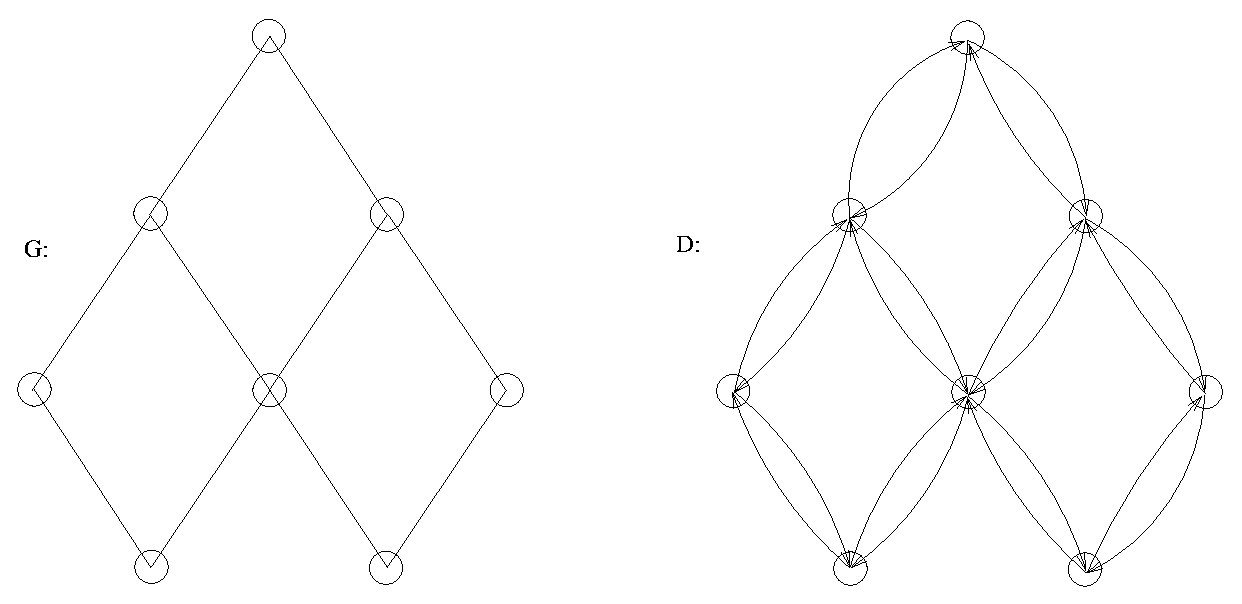
\includegraphics[scale=0.55]{figures/digrafo_ini.eps}
\label{fig:fig1}
\end{figure}

\end{frame}

\begin{frame}{Subgrafo enraizado em $r$}
  \begin{itemize}
  \item $r \in V$.
    \\$z^{r} = (z_{ij}^{r})_{ij \in A}$.
  %% \item Seja $x \in \espacoXBinary$. Para cada~$e \in E$, \hbox{$x(e) = 1$} sse $e$ faz parte da solução.    
  \end{itemize}

\begin{lpformulation}[]
    \lpeq[]{\sum_{i \in \delta^{-}(j)}z^{r}_{ij} = 1}{r \in V,\,\forall j \in V \setminus \{r\}}
    \lpeq[]{\sum_{i \in \delta^{-}(r)}z^{r}_{ir} = 0}{r \in V}
    \lpeq[]{z^{r} \in \espacoZBinary}{r \in V}
\lplabel{lp:tree_restriction}
\end{lpformulation}
\end{frame}

\begin{frame}{Subgrafo formado pelos arcos selecionados \hyperlink{rel_subgrafos}{\beamergotobutton{$\leftarrow$}}}
  \hypertarget{arb_diferentes}{}
  \begin{figure}[H]
\centering
%\input{figures/xfig/arb_diferentes}
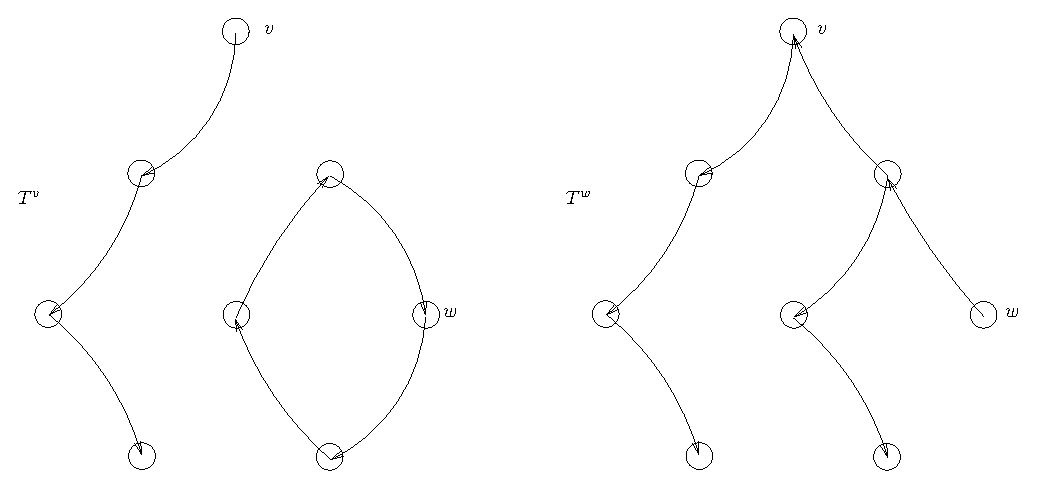
\includegraphics[scale=0.55]{figures/arb_diferentes.eps}
\label{fig:fig1}
  \end{figure}

\begin{fato}
  \label{afirm:num_arcos}
  Para cada $v \in V$, o subgrafo $T^{v}$ tem exatamente $|V| - 1$ arcos.
\end{fato}
  
\end{frame}


%% \begin{frame}{Quantidade de arcos}
%%   \begin{itemize}
%%   \item Seja $\tilde{z}^{v}$ um ponto que satisfaz o sistema anterior.
%%   \item Seja $T^{v} \subseteq D$ t.q. $A(T^{v}) = \{ ij \in A: \tilde{z}_{ij}^{v} = 1 \}$
%% \begin{fato}
%%   \label{afirm:num_arcos}
%%   O subgrafo $T^{v}$ tem exatamente $|V| - 1$ arcos.
%% \end{fato}
    
%%   \end{itemize}
%% \end{frame}

\begin{frame}{Relacionando os subgrafos $T^{r}$}
  \begin{itemize}
  \item $x \in \espacoXBinary$. \\
    Para cada~$e \in E$, \hbox{$x(e) = 1$} sse $e$ faz parte da solução.

    \begin{align}
      &\sum_{i \in \delta^{-}(j)}z^{r}_{ij} = 1 && \forall r \in V,\,\forall j \in V \setminus \{r\} \nonumber\\
      &\sum_{i \in \delta^{-}(r)}z^{r}_{ir} = 0 && \forall r \in V\nonumber\\
      &\textcolor{red}{x_{e} = z^{r}_{ij} + z^{r}_{ji}} && \textcolor{red}{\forall r \in V,\, \forall e = \{i,j\} \in E}\\
      &\textcolor{red}{x \in \espacoXBinary}, z^{r} \in \espacoZBinary && \forall r \in V
    \end{align}
    
    %% \begin{lpformulation}[]
    %%   \lpeq*[]{\sum_{i \in \delta^{-}(j)}z^{r}_{ij} = 1}{r \in V,\,\forall j \in V \setminus \{r\}}
    %%   \lpeq*[]{\sum_{i \in \delta^{-}(r)}z^{r}_{ir} = 0}{r \in V}
    %%   \lpeq[]{x_{e} = z^{r}_{ij} + z^{r}_{ji}}{r \in V,\, \forall e = \{i,j\} \in E}
    %%   \lpeq[]{x \in \espacoXBinary, z^{r} \in \espacoZBinary}{r \in V}      
    %%   \lplabel{lp:tree_restriction}
    %% \end{lpformulation}      
  \end{itemize}
\end{frame}

\begin{frame}{Relacionando os subgrafos $T^{r}$ \hyperlink{arb_diferentes}{\beamergotobutton{ex}}}
  \hypertarget{rel_subgrafos}{}
  \begin{itemize}
  \item $(x,\tilde{z})$ solução do sistema anterior.
  \item Para $v \in V$, $T^{v} \subseteq D$ t.q. $A(T^{v}) = \{ ij \in A: \tilde{z}_{ij}^{v} = 1 \}$.
  \item 
    $\widetilde{T}^{v} \subseteq G$ o grafo subjacente
    a $T^{v}$ t.q. \mbox{$E(\widetilde{T}^{v}) = \{ij \in E: ij \in T^{v} \text{ ou }ji \in T^{v}\}$}.\\

    %$\widetilde{T}^{v} = \widetilde{T}^{w}$, $\forall v, w \in V$;

\begin{align*}
  \widetilde{T}^{v} = \widetilde{T}^{w}, \: \forall v, w \in V;
\end{align*}

  \item $T^{v}$ é uma \textcolor{red}{arborescência} de $D$, com raiz $v$, $\forall v \in V$.
%% \begin{fato}
%%   \label{afirm:arv_geradora}
%%   Seja $T \subseteq G$ tal que $E(T) = \{e \in E: x_e = 1\}$. Então $T$
%%   é uma árvore geradora de~$G$, e $T=\widetilde{T}^{v}$ para todo
%%   $v\in V$.
%% \end{fato}
    
%% \begin{align}
%%   \label{afirm:arborescence}
%%   T^{v} \text{ é uma arborescência de }D, \text{ com raiz }v, \: \forall v \in V.
%% \end{align}

  \end{itemize}
  
\end{frame}


\begin{frame}{Arborescências se sobrepondo \hyperlink{form_1}{\beamergotobutton{$\leftarrow$}}}
  \hypertarget{arb_iguais}{}
  \begin{figure}[H]
\centering
%\input{figures/xfig/arb_diferentes}
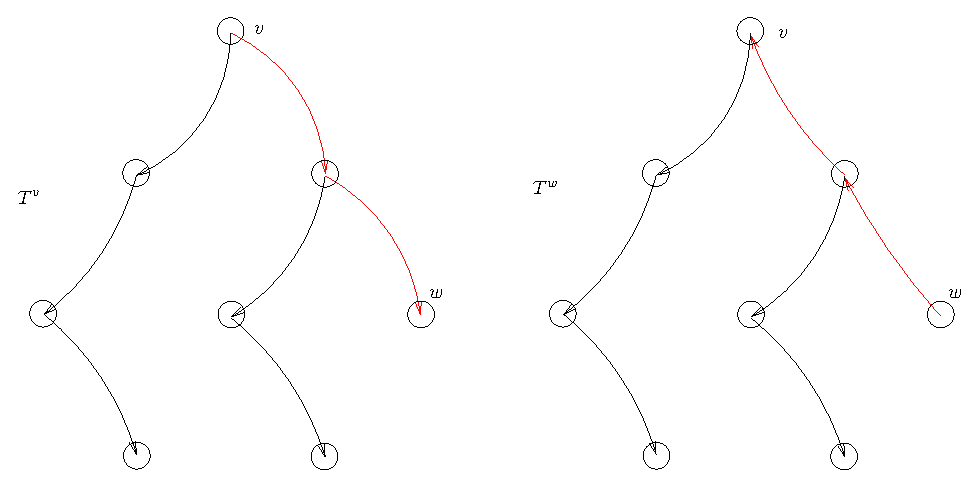
\includegraphics[scale=0.55]{figures/arb_iguais.eps}
\label{fig:fig1}
\end{figure}
\end{frame}

\begin{frame}{Variável que representa distância \hyperlink{sig_u}{\beamergotobutton{sig. u}}}
  \hypertarget{var_u}{}
  \begin{itemize}
  \item $r \in V$, $u^{r} \in \espacoUr$. \\
  \item Para cada $i \in V:$\\
    \textcolor{red}{$u^{r}_{i}$}: distância entre $r$ e $i$ em $T^{r}$.\\
    $M_{ij}^{r}:$ limite superior para $u^{r}_{i} - u^{r}_{j}$.
  \item Fixe $r:$
 %\end{itemize}

%% \begin{block}{concretization}
%%   \renewcommand{\arraystretch}{1.5}%
%%   \resizebox{!}{5mm}{% Height of 5mm; maintain aspect ratio    
%%   }
%% \end{block}

{\tiny
  \begin{lpformulation}[]
    \lpeq[res:mtz_var]{u_{i} - u_{j} + (M_{ij} + w_{ij}) z_{ij} + (M_{ij} -w_{ij})z_{ji} \le M_{ij}}{ij \in A, j \ne r}
    \lpeq[]{u_{i} + (M_{ir} -w_{ir})z_{ri} \le M_{ir}}{ri \in A}    
  \end{lpformulation}    
  
  }

%% \resizebox{.9 \textwidth}{!} 
%% {
%% }
    
%% \tiny{%
%%   \vbox{%
%%  }} 
     
\item
  %<4-> Validade da inequação \ref{res:mtz_var}:\\
  %%   $z_{ij} = 1, z_{ji} = 0 \Rightarrow u_j \ge u_i + w_{ij}$\\
  %% $z_{ij} = 0, z_{ji} = 1 \Rightarrow u_i - u_j \le w_{ij}$ \\
  $z_{ij} = 0, z_{ji} = 0 \Rightarrow u_i - u_j \le M_{ij}$ 
  
  \end{itemize}

\end{frame}


\begin{frame}{Significado da variável $u^{r}$ \hyperlink{var_u}{\beamergotobutton{$\leftarrow$}}}
  \hypertarget{sig_u}{}
  \begin{figure}[H]
\centering
%\input{figures/xfig/arb_diferentes}
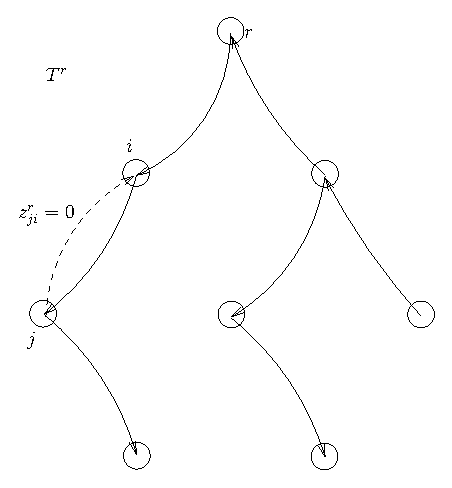
\includegraphics[scale=0.45]{figures/variavel_u.eps}
\label{fig:fig1}
  \end{figure}

  {\footnotesize
  \begin{itemize}

  \item Ineq. \ref{res:mtz_var} com relação ao arco $ij:$
    \begin{align*}
  u^{r}_i - u^{r}_j + (M^{r}_{ij} + w_{ij}) \cdot 1 + (M^{r}_{ij} - w_{ij}) \cdot 0 \le M^{r}_{ij} \Rightarrow u^{r}_j \ge u^{r}_i + w_{ij}.
\end{align*}
    
  \item Ineq. \ref{res:mtz_var} com relação ao arco $ji:$
    \begin{align*}
  u^{r}_j - u^{r}_i + (M^{r}_{ji} + w_{ij}) \cdot 0 + (M^{r}_{ji} - w_{ij}) \cdot 1 \le M^{r}_{ji} \Rightarrow u^{r}_j \le u^{r}_i + w_{ij}.
\end{align*}

\begin{align*}
  u^{r}_j = u^{r}_i + w_{ij}.
\end{align*}

    
  \end{itemize}
}
  
\end{frame}


\begin{frame}{Formulação: variáveis que representam distâncias}
  \tiny
  \Fontvi
  \begin{lpformulation} %[{\rm (PI)}]
    \lpobj*{min}{\sum_{e\in E} w_ex_e}
    \lpeq*[]{\sum_{i \in \delta^{-}(j)}z^{r}_{ij} = 1}{r \in V,\,\forall j \in V \setminus \{r\}}
    \lpeq*[]{\sum_{i \in \delta^{-}(r)}z^{r}_{ir} = 0}{r \in V}
    \lpeq*[]{\sum_{e \in E}x_e = |V| - 1}{}
    \lpeq*[]{x_{e} = z^{r}_{ij} + z^{r}_{ji}}{r \in V,\, \forall e = \{i,j\} \in E}
    \lpeq*[]{u^{r}_{i} - u^{r}_{j} + (M_{ij} + w_{ij}) z^{r}_{ij} + (M_{ij} -w_{ij})z^{r}_{ji} \le M_{ij}}{r \in V, \forall ij \in A, j \ne r}
    \lpeq*[]{u^{r}_{i} + (M_{ir} -w_{ir})z_{ri} \le M_{ir}}{r \in V, \forall ri \in A}
    %\lpeq[]{u^{r}_{r} = 0}{r \in V}
    \lpeq*[]{u^{j}_{i} = u^{i}_{j} \le t \cdot w_{ij}}{ij \in E}
    \lpeq*[]{x \in \espacoXBinary, z^{r} \in \espacoZBinary, u^{r} \in \espacoUuni}{r \in V}
\end{lpformulation}
  
\end{frame}

\section{Experimentos}

\begin{frame}{Custos representando distância euclidiana}
%\begin{center}
%\noindent
  \tiny{
    \Fontvi
\begin{table}
\begin{tabular}{|c|c|c|c|r|c|r|c|}\hline

{$t$} & {$|V|$} & {Densidade (\%)} & {\# Resolvido } & {Tempo (s)}  &{\# Árvore}  &{Tempo (s)} & {Gap}
\\ \hline\hline
%\multirow{2}{*}{3} & 10 & 40 & 5 (3) & 0(23) & 0.02(0.09) & 0.02(3.87) & 3(2.32)\\
3 & 10 & 20 & 10 (10) & 0.01 (0.01) & 10 (10) & 0.01 (0.01) & 1.00 \\
 & 20 & & 10 (10) & 0.08 (0.06) & 4 (8) & 0.13 (0.06) & 1.00 \\
 & 30 & & 10 (10) & 0.25 (0.35) & 0 (6) & - (0.49) & - \\
 & 40 & & 10 (10) & 0.50 (1.31) & 0 (5) & - (2.28) & - \\
 & 48 & & 10 (10) & 1.09 (4.37) & 0 (5) & - (8.03) & - \\
 & 20 & 40 & 10 (10) & 0.27 (0.28) & 3 (10) & 0.45 (0.28) & 1.01 \\
 & 30 & & 10 (10) & 0.64 (2.29) & 0 (10) & - (2.29) & - \\
 & 40 & & 10 (10) & 1.75 (18.63) & 0 (8) & - (23.10) & - \\
 & 48 & & 10 (10) & 3.20 (67.92) & 0 (6) & - (112.22) & - \\
 & 20 & 60 & 10 (10) & 0.36 (0.58) & 4 (10) & 0.53 (0.58) & 1.00 \\
 & 30 & & 10 (10) & 1.64 (9.92) & 2 (10) & 2.77 (9.92) & 1.02 \\
 & 40 & & 10 (10) & 4.02 (90.37) & 0 (10) & - (90.37) & - \\
 & 48 & & 10 (10) & 9.28 (1040.88) & 0 (10) & - (1040.88) & - \\
 & 20 & 80 & 10 (10) & 1.27 (1.60) & 9 (10) & 1.36 (1.60) & 1.01 \\
 & 30 & & 10 (10) & 3.56 (75.45) & 2 (10) & 8.71 (75.45) & 1.04 \\
 & 40 & & 10 (10) & 7.72 (308.18) & 0 (10) & - (308.18) & - \\
 & 48 & & 10 (5) & 15.64 (1336.80) & 0 (5) & - (1336.80) & - \\
4 & 20 & 20 & 10 (10) & 0.21 (0.06) & 10 (10) & 0.21 (0.06) & 1.01 \\
 & 30 & & 10 (10) & 1.25 (0.45) & 7 (10) & 1.57 (0.45) & 1.03 \\
 & 40 & & 10 (10) & 2.55 (2.52) & 3 (10) & 4.57 (2.52) & 1.02 \\
 & 48 & & 10 (10) & 11.50 (9.11) & 4 (10) & 19.31 (9.11) & 1.01 \\
 & 20 & 40 & 10 (10) & 0.73 (0.23) & 10 (10) & 0.73 (0.23) & 1.00 \\
 & 30 & & 10 (10) & 6.69 (3.95) & 9 (10) & 7.17 (3.95) & 1.03 \\
 & 40 & & 10 (10) & 137.60 (46.20) & 9 (10) & 108.58 (46.20) & 1.02 \\
 & 48 & & 10 (10) & 597.27 (193.89) & 4 (10) & 851.26 (193.89) & 1.03 \\
 & 20 & 60 & 10 (10) & 1.30 (0.37) & 10 (10) & 1.30 (0.37) & 1.00 \\
 & 30 & & 10 (10) & 37.22 (10.56) & 10 (10) & 37.22 (10.56) & 1.02 \\
 & 40 & & 9 (10) & 888.34 (167.80) & 9 (10) & 888.34 (167.80) & 1.05 \\
 & 48 & & 4 (10) & 299.92 (1194.66) & 1 (10) & 569.29 (1194.66) & 1.05 \\
 & 20 & 80 & 10 (10) & 1.89 (0.68) & 10 (10) & 1.89 (0.68) & 1.01 \\
 & 30 & & 10 (10) & 81.62 (52.53) & 9 (10) & 87.28 (52.53) & 1.01 \\
 & 40 & & 2 (10) & 1457.22 (477.65) & 2 (10) & 1457.22 (477.65) & 1.02 \\
\rowcolor[rgb]{1,1,0} & 48 & & 0 (3) & - (2137.70) & 0 (3) & - (2137.70) & - \\

\hline\hline
\end{tabular}
\end{table}
}
%% \captionof{table}{Computational results for the cardinality version}\label{tab:exec_time}
%\end{center}
  
\end{frame}

\begin{frame}{Custos representando distância euclidiana}
%\begin{center}
%\noindent
  \tiny{
    \Fontvi
\begin{table}
\begin{tabular}{|c|c|c|>{\columncolor[rgb]{1,1,0}}c|r|>{\columncolor[rgb]{1,1,0}}c|r|c|}\hline

{$t$} & {$|V|$} & {Densidade (\%)} & {\# Resolvido } & {Tempo (s)}  &{\# Árvore}  &{Tempo (s)} & {Gap}
\\ \hline\hline

5 & 20 & 20 & 10 (10) & 0.28 (0.06) & 10 (10) & 0.28 (0.06) & 1.00 \\
 & 30 & & 10 (10) & 2.58 (0.42) & 10 (10) & 2.58 (0.42) & 1.00 \\
 & 40 & & 10 (10) & 71.07 (1.98) & 10 (10) & 71.07 (1.98) & 1.01 \\
 & 48 & & 9 (10) & 899.04 (7.19) & 9 (10) & 899.04 (7.19) & 1.01 \\
 & 20 & 40 & 10 (10) & 0.85 (0.19) & 10 (10) & 0.85 (0.19) & 1.00 \\
 & 30 & & 10 (10) & 9.99 (1.52) & 10 (10) & 9.99 (1.52) & 1.00 \\
 & 40 & & 10 (10) & 407.52 (22.62) & 10 (10) & 407.52 (22.62) & 1.00 \\
 & 48 & & 5 (10) & 707.52 (112.32) & 5 (10) & 707.52 (112.32) & 1.00 \\
 & 20 & 60 & 10 (10) & 1.78 (0.35) & 10 (10) & 1.78 (0.35) & 1.00 \\
 & 30 & & 10 (10) & 87.97 (4.51) & 10 (10) & 87.97 (4.51) & 1.00 \\
 & 40 & & 6 (10) & 837.34 (103.33) & 6 (10) & 837.34 (103.33) & 1.01 \\
 & 48 & & 3 (10) & 1327.73 (954.20) & 3 (10) & 1327.73 (954.20) & 1.00 \\
 & 20 & 80 & 10 (10) & 1.96 (0.58) & 10 (10) & 1.96 (0.58) & 1.00 \\
 & 30 & & 10 (10) & 144.77 (16.36) & 10 (10) & 144.77 (16.36) & 1.01 \\
 & 40 & & 3 (10) & 592.59 (383.50) & 3 (10) & 592.59 (383.50) & 1.00 \\
\rowcolor[rgb]{1,1,0} & 48 & & 1 (6) & 654.22 (1299.59) & 1 (6) & 654.22 (1299.59) & 1.00 \\
6 & 20 & 20 & 10 (10) & 0.30 (0.06) & 10 (10) & 0.30 (0.06) & 1.00 \\
 & 30 & & 10 (10) & 1.78 (0.35) & 10 (10) & 1.78 (0.35) & 1.00 \\
 & 40 & & 10 (10) & 16.10 (1.77) & 10 (10) & 16.10 (1.77) & 1.00 \\
 & 48 & & 10 (10) & 66.69 (5.79) & 10 (10) & 66.69 (5.79) & 1.00 \\
 & 20 & 40 & 10 (10) & 0.71 (0.16) & 10 (10) & 0.71 (0.16) & 1.00 \\
 & 30 & & 10 (10) & 4.71 (1.53) & 10 (10) & 4.71 (1.53) & 1.00 \\
 & 40 & & 10 (10) & 41.03 (13.66) & 10 (10) & 41.03 (13.66) & 1.00 \\
 & 48 & & 6 (10) & 381.58 (92.55) & 6 (10) & 381.58 (92.55) & 1.00 \\
 & 20 & 60 & 10 (10) & 1.32 (0.31) & 10 (10) & 1.32 (0.31) & 1.00 \\
 & 30 & & 10 (10) & 15.31 (3.31) & 10 (10) & 15.31 (3.31) & 1.00 \\
 & 40 & & 10 (10) & 312.66 (71.21) & 10 (10) & 312.66 (71.21) & 1.00 \\
 & 48 & & 4 (10) & 883.03 (645.75) & 4 (10) & 883.03 (645.75) & 1.00 \\
 & 20 & 80 & 10 (10) & 1.57 (0.51) & 10 (10) & 1.57 (0.51) & 1.00 \\
 & 30 & & 10 (10) & 31.24 (13.04) & 10 (10) & 31.24 (13.04) & 1.00 \\
 & 40 & & 8 (10) & 745.06 (309.45) & 8 (10) & 745.06 (309.45) & 1.00 \\
\rowcolor[rgb]{1,1,0} & 48 & & 2 (6) & 1929.29 (1733.04) & 2 (6) & 1929.29 (1733.04) & 1.00 \\

\hline\hline
\end{tabular}
\end{table}
}
%% \captionof{table}{Computational results for the cardinality version}\label{tab:exec_time}
%\end{center}
  
\end{frame}


\begin{frame}{Arestas com custo unitário}
%\begin{center}
%\noindent
  \tiny{
    \Fontvi
\begin{table}
\begin{tabular}{|c|c|c|c|r|c|r|}\hline

{$t$} & {$|V|$} & {Densidade (\%)} & {\# Resolvido } & {Tempo (s)}  &{\# Árvore}  &{Tempo (s)} 
\\ \hline\hline

3 & 20 & 20 & 10 (10) & 0.085 (0.116) & 0 (8) & - (0.136) \\ 
 & 30 & & 10 (10) & 0.450 (2.452) & 0 (10) & - (2.452) \\ 
 & 40 & & 10 (10) & 133.422 (50.835) & 0 (10) & - (50.835) \\ 
 & 50 & & 7 (10) & 5.977 (407.598) & 0 (10) & - (407.598) \\ 
 & 60 & & 9 (10) & 13.384 (1527.632) & 0 (10) & - (1527.632) \\ 
 & 20 & 40 & 10 (10) & 10.962 (0.589) & 0 (10) & - (0.589) \\ 
 & 30 & & 10 (10) & 1968.557 (18.628) & 1 (10) & 1208.580 (18.628) \\ 
 & 40 & & - (10) & - (327.345) & - (10) & - (327.345) \\ 
 \rowcolor[rgb]{1,1,0}& 50 & & - (8) & - (1995.574) & - (8) & - (1995.574) \\ 
% & 60 & & - (-) & - (-) & - (-) & - (-) \\ 
 & 20 & 60 & 10 (10) & 71.356 (1.058) & 8 (10) & 59.360 (1.058) \\ 
 & 30 & & 6 (10) & 1882.148 (40.350) & 5 (10) & 1557.828 (40.350) \\ 
 & 40 & & - (10) & - (1797.575) & - (10) & - (1797.575) \\ 
 & 50 & & - (-) & - (-) & - (-) & - (-) \\ 
% & 60 & & - (-) & - (-) & - (-) & - (-) \\ 
 & 20 & 80 & 10 (10) & 82.841 (2.595) & 10 (10) & 82.841 (2.595) \\ 
 & 30 & & 10 (10) & 1335.604 (97.473) & 10 (10) & 1335.604 (97.473) \\ 
 & 40 & & - (7) & - (2588.981) & - (7) & - (2588.981) \\ 
 & 50 & & - (-) & - (-) & - (-) & - (-) \\ 
% & 60 & & - (-) & - (-) & - (-) & - (-) \\ 
4 & 20 & 20 & 10 (10) & 4.674 (0.152) & 4 (10) & 5.655 (0.152) \\ 
 & 30 & & 4 (10) & 496.532 (2.710) & 0 (10) & - (2.710) \\ 
 & 40 & & - (10) & - (52.355) & - (10) & - (52.355) \\ 
 & 50 & & - (10) & - (446.987) & - (10) & - (446.987) \\ 
 & 60 & & - (10) & - (1763.765) & - (10) & - (1763.765) \\ 
 & 20 & 40 & 10 (10) & 25.003 (0.558) & 10 (10) & 25.003 (0.558) \\ 
 & 30 & & 8 (10) & 1019.185 (18.965) & 8 (10) & 1019.185 (18.965) \\ 
 & 40 & & 4 (10) & 2332.998 (335.994) & 4 (10) & 2332.998 (335.994) \\ 
 & 50 & & - (9) & - (1975.087) & - (9) & - (1975.087) \\ 
% & 60 & & - (-) & - (-) & - (-) & - (-) \\ 
 & 20 & 60 & 10 (10) & 29.279 (1.140) & 10 (10) & 29.279 (1.140) \\ 
 & 30 & & 10 (10) & 625.866 (42.766) & 10 (10) & 625.866 (42.766) \\ 
 & 40 & & - (9) & - (1281.802) & - (9) & - (1281.802) \\ 
 & 50 & & - (-) & - (-) & - (-) & - (-) \\ 
% & 60 & & - (-) & - (-) & - (-) & - (-) \\ 
 & 20 & 80 & 10 (10) & 48.525 (2.927) & 10 (10) & 48.525 (2.927) \\ 
 & 30 & & 10 (10) & 721.166 (106.070) & 10 (10) & 721.166 (106.070) \\ 
 & 40 & & 1 (8) & 536.152 (2326.041) & 1 (8) & 536.152 (2326.041) \\ 
 & 50 & & - (-) & - (-) & - (-) & - (-) \\ 
% & 60 & & - (-) & - (-) & - (-) & - (-) \\ 


\hline\hline
\end{tabular}
\end{table}
}
%% \captionof{table}{Computational results for the cardinality version}\label{tab:exec_time}
%\end{center}
  
\end{frame}


\begin{frame}{Arestas com custo unitário}
%\begin{center}
%\noindent
  \tiny{
    \Fontvi
\begin{table}
\begin{tabular}{|c|c|c|>{\columncolor[rgb]{1,1,0}}c|r|>{\columncolor[rgb]{1,1,0}}c|r|}\hline

{$t$} & {$|V|$} & {Densidade (\%)} & {\# Resolvido } & {Tempo (s)}  &{\# Árvore}  &{Tempo (s)} 
\\ \hline\hline

5 & 20 & 20 & 10 (10) & 1.414 (0.151) & 10 (10) & 1.414 (0.151) \\ 
 & 30 & & 10 (10) & 497.008 (2.757) & 10 (10) & 497.008 (2.757) \\ 
 & 40 & & 3 (10) & 1400.120 (50.026) & 3 (10) & 1400.120 (50.026) \\ 
 & 50 & & - (10) & - (422.061) & - (10) & - (422.061) \\ 
 & 60 & & - (10) & - (1908.589) & - (10) & - (1908.589) \\ 
 & 20 & 40 & 10 (10) & 1.733 (0.576) & 10 (10) & 1.733 (0.576) \\ 
 & 30 & & 10 (10) & 229.043 (20.892) & 10 (10) & 229.043 (20.892) \\ 
 & 40 & & 4 (10) & 2112.543 (305.310) & 4 (10) & 2112.543 (305.310) \\ 
 \rowcolor[rgb]{1,1,0}& 50 & & - (10) & - (1812.215) & - (10) & - (1812.215) \\ 
% & 60 & & - (-) & - (-) & - (-) & - (-) \\ 
 & 20 & 60 & 10 (10) & 16.679 (1.087) & 10 (10) & 16.679 (1.087) \\ 
 & 30 & & 10 (10) & 508.871 (46.154) & 10 (10) & 508.871 (46.154) \\ 
 & 40 & & - (10) & - (1270.654) & - (10) & - (1270.654) \\ 
 & 50 & & - (1) & - (3064.760) & - (1) & - (3064.760) \\ 
% & 60 & & - (-) & - (-) & - (-) & - (-) \\ 
 & 20 & 80 & 10 (10) & 51.066 (2.539) & 10 (10) & 51.066 (2.539) \\ 
 & 30 & & 10 (10) & 1074.430 (130.023) & 10 (10) & 1074.430 (130.023) \\ 
 & 40 & & - (9) & - (2318.212) & - (9) & - (2318.212) \\ 
 & 50 & & - (-) & - (-) & - (-) & - (-) \\ 
% & 60 & & - (-) & - (-) & - (-) & - (-) \\ 
6 & 20 & 20 & 10 (10) & 0.532 (0.154) & 10 (10) & 0.532 (0.154) \\ 
 & 30 & & 10 (10) & 24.199 (2.684) & 10 (10) & 24.199 (2.684) \\ 
 & 40 & & 7 (10) & 756.216 (52.941) & 7 (10) & 756.216 (52.941) \\ 
 & 50 & & 3 (10) & 3228.030 (473.483) & 3 (10) & 3228.030 (473.483) \\ 
 & 60 & & - (10) & - (1586.939) & - (10) & - (1586.939) \\ 
 & 20 & 40 & 10 (10) & 0.126 (0.667) & 10 (10) & 0.126 (0.667) \\ 
 & 30 & & 10 (10) & 32.169 (21.069) & 10 (10) & 32.169 (21.069) \\ 
 & 40 & & 10 (10) & 969.422 (384.778) & 10 (10) & 969.422 (384.778) \\ 
 & 50 & & 1 (9) & 1660.530 (2035.015) & 1 (9) & 1660.530 (2035.015) \\ 
% & 60 & & - (-) & - (-) & - (-) & - (-) \\ 
 & 20 & 60 & 10 (10) & 1.529 (1.082) & 10 (10) & 1.529 (1.082) \\ 
 & 30 & & 10 (10) & 145.620 (44.354) & 10 (10) & 145.620 (44.354) \\ 
 & 40 & & 6 (10) & 2842.812 (1131.076) & 6 (10) & 2842.812 (1131.076) \\ 
 & 50 & & - (2) & - (2441.080) & - (2) & - (2441.080) \\ 
% & 60 & & - (-) & - (-) & - (-) & - (-) \\ 
 & 20 & 80 & 10 (10) & 2.787 (2.647) & 10 (10) & 2.787 (2.647) \\ 
 & 30 & & 10 (10) & 118.607 (108.115) & 10 (10) & 118.607 (108.115) \\ 
 & 40 & & 8 (8) & 683.165 (2321.856) & 8 (8) & 683.165 (2321.856) \\ 
 & 50 & & - (-) & - (-) & - (-) & - (-) \\ 
% & 60 & & - (-) & - (-) & - (-) & - (-) \\ 


\hline\hline
\end{tabular}
\end{table}
}
%% \captionof{table}{Computational results for the cardinality version}\label{tab:exec_time}
%\end{center}
  
\end{frame}

\begin{frame}
  Muito obrigado!
\end{frame}

\begin{frame}{Formulação 2: Encontrando distâncias entre vértices \hyperlink{arb_iguais}{\beamergotobutton{ex}} \hyperlink{sig_y}{\beamergotobutton{sig. y}}}
  \hypertarget{form_1}{}
  \tiny
  \Fontvi
  \begin{lpformulation} %[{\rm (1)}]
    \lpobj*{min}{\sum_{e\in E} w_ex_e}
    \lpeq[]{\sum_{i \in \delta^{-}(j)}z^{r}_{ij} = 1}{r \in V,\,\forall j \in V \setminus \{r\}}
    \lpeq[]{\sum_{i \in \delta^{-}(r)}z^{r}_{ir} = 0}{r \in V}
    \lplabel{lp:tree_restriction}
    \lpeq[res_mwstp:num_aresta]{\sum_{e \in E}x_e = |V| - 1}{}
    \lpeq[]{x_{e} = z^{r}_{ij} + z^{r}_{ji}}{r \in V,\, \forall e = \{i,j\} \in E}
    \lpeq[]{z^{u}_{ij} - z^{v}_{ij} \le y^{uv}_{e} \le z^{u}_{ij} + z^{v}_{ij}} {uv \in E,\, \forall e = \{i,j\} \in E}
    \lpeq[]{z^{u}_{ji} - z^{v}_{ji} \le y^{uv}_{e} \le z^{u}_{ji} + z^{v}_{ji}} {uv \in E,\, \forall e = \{i,j\} \in E}
    \lpeq[res_mwsp:single_in-arc]{\sum_{e \in E} w^{}_e\,y^{uv}_{e} \le t \cdot w_{uv}}{uv \in E}
    \lpeq[]{x \in \espacoXBinary, y \in \espacoZBinary, z^{v} \in \espacoZBinary}{v \in V}
\end{lpformulation}  
\end{frame}


\begin{frame}{Significado da variável $y$ \hyperlink{form_1}{\beamergotobutton{$\leftarrow$}}}
  \hypertarget{sig_y}{}
  {\footnotesize
  \begin{itemize}
    \item Para todo $u,v \in V$, seja $T_{u,v}$ o caminho entre $u$ e $v$ em $T$.
    \item Para todo $uv,ij \in E$:
  \end{itemize}
\begin{align*}
  d^{u v}_{ij} := z^{u}_{ij} - z^{v}_{ij}\\
  s^{u v}_{ij} := z^{u}_{ij} + z^{v}_{ij}\\
  \end{align*}

%\small
\begin{center}
  \noindent
  %\captionof{table}{Diferenças e somas relativas à variável $z$}
  \label{tab:sum_diff} 
\begin{tabular}{|r|r|r|r|}\hline
{$d^{uv}_{ij}$ $s^{uv}_{ij}$} & {$z^{u}_{ij}$ $z^{v}_{ij}$} & {$z^{u}_{ji}$ $z^{v}_{ji}$} & {$d^{uv}_{ji}$ $s^{uv}_{ji}$}
\\ \hline\hline 
$1\quad 1$ & $1\quad 0$ & $0\quad 1$ & $-1\quad 1$ \\
$-1\quad 1$ & $0\quad 1$ & $1\quad 0$ & $1\quad 1$ \\
$0\quad 2$ & $1\quad 1$ & $0\quad 0$ & $0\quad 0$ \\
$0\quad 0$ & $0\quad 0$ & $1\quad 1$ & $0\quad 2$ \\
$0\quad 0$ & $0\quad 0$ & $0\quad 0$ & $0\quad 0$ \\
\hline\hline
\end{tabular}
\end{center}


\begin{lpformulation}[]
  \lpeq[res_mwstp:define_y_ij]{d^{uv}_{ij} \le y^{uv}_{e} \le s^{uv}_{ij}} {uv \in E, \forall e = \{i,j\} \in E}
  \lpeq[res_mwstp:define_y_ji]{d^{uv}_{ji} \le y^{uv}_{e} \le s^{uv}_{ji}} {uv \in E, \forall e = \{i,j\} \in E}
\end{lpformulation}

\begin{align}
  \label{afirm:valor_y}
  y^{uv}_e = 1 \Leftrightarrow e \in T_{u,v}.
\end{align}
}

\end{frame}

\begin{frame}{Definições equivalentes de spanner \hyperlink{span}{\beamergotobutton{$\leftarrow$}}}
  \hypertarget{def_span}{}
  \begin{itemize}
    \item Afirmações equivalentes:
      \begin{itemize}
        \item[{\rm (a)}] $H$ é um $t$-spanner de $G$, isto é, $H$ satisfaz (\ref{eq:def_spanner});
        \item[{\rm (b)}] $\dist_{H}(u,v) \le t \cdot \dist_{G}(u,v) \;\forall\,uv \in E$;
        \item[{\rm (b')}] $\dist_{H}(u,v) \le t \cdot \dist_{G}(u,v) \;\forall\,uv \in E \setminus E(H)$;
        \item[{\rm (c)}] $\dist_{H}(u,v) \le t \cdot w_{uv} \;\forall\,uv \in E$.
        \item[{\rm (c')}] $\dist_{H}(u,v) \le t \cdot w_{uv} \;\forall\,uv \in E \setminus E(H)$.
        \end{itemize}
    \end{itemize}
\end{frame}


\bibliographystyle{sbc}
\bibliography{talk}

\end{document}
